\section{BJT(Transistore bipolare a giunzione)}

Il BJT è un tripolo(diodo a tre terminazioni):
\begin{itemize}
    \item collettore
    \item base 
    \item emettitore
\end{itemize}

\begin{figure}[H]
    \centering
    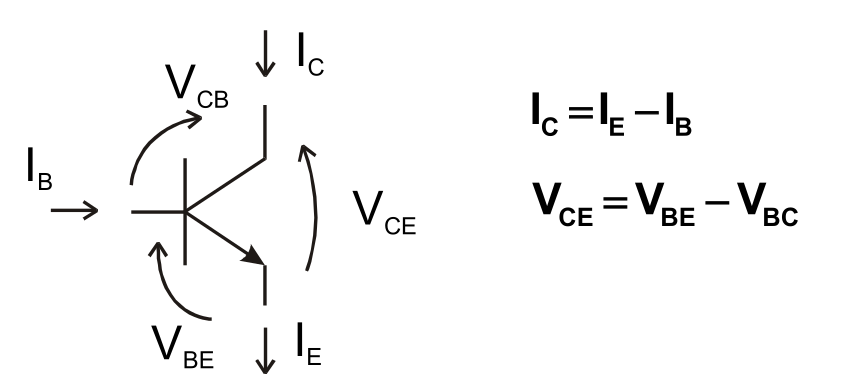
\includegraphics[width=0.5\linewidth]{2 - dispositivi elettronici/imgs/Screenshot from 2022-06-14 23-14-03.png}
    \label{fig:BJT}
    \caption{Diodo BJT}
\end{figure}

\subsection{Zone di funzionamento}

\begin{figure}[H]
    \centering
    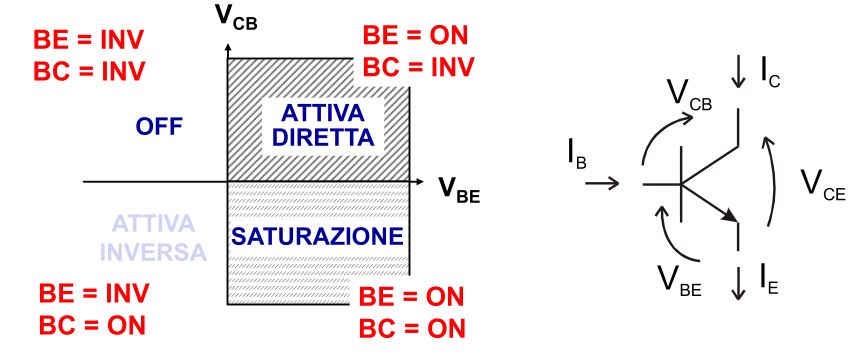
\includegraphics[width=0.5\linewidth]{2 - dispositivi elettronici/imgs/Screenshot from 2022-06-14 23-16-33.png}
    \label{fig:BJT_funzionamento}
    \caption{Funzionamento BJT}
\end{figure}

\subsubsection{Zona attiva diretta}
la corrente di base(di solito piccola) funge da controllo rispetto alla corrente (solitamente enorme) sul collettore.

\subsubsection{Zona di saturazione}
In questo caso la base funge da interruttore, o passa 0 corrente o passa tutta la corrente tra collettore ed emettitore.

\section{da riguardare il BJT per gli esercizi}